\chapter{Introduction into \parref{par:three}}

In \parref{par:three} we provide a more general discussion of tensor calculus, which has been applied in \parref{par:one} and \parref{par:two}.
Since the contraction operation is central in these calculus schemes, we refer to the set of techniques as contraction calculus.

\sect{Encoding schemes for functions}

\textbf{One-hot encodings} are the central encoding schemes of states in factored system representations.
As will be presented in more detail in \charef{cha:coordinateCalculus}, they build a basis of the tensor space.
We use one-hot encodings in the construction of further encoding schemes of functions on the set of states in factored system representations.

\textbf{\CoordinateEncoding{}s} use the real coordinates multiplying each one-hot encoding to store information.
They have implicitly been used in the representation of factored systems in \parref{par:one}, where probability distributions and logical formulas have been treated as tensors.
More precise, these tensors are the coordinate encodings of probability distributions and logical formulas, which are maps of the state set into the interval $[0,1]$ and into the set $\ozset$.

\textbf{\BasisEncoding{}s} are sums of a collection of one-hot encodings.
They differ from coordinate encodings that they do not allow weights by general real numbers in these sums, and restrict to booleans.
Basis encodings therefore map the set of subsets to an enumerated set bijectively onto the set of boolean tensors.
We introduce them in \charef{cha:basisCalculus} in most generality as an encoding scheme for subsets of enumerated set, which we then extend towards relations and functions.
The main advantage of basis encodings is the efficient representation of function compositions by tensor networks of basis encodings.
This scheme is the main representation paradigm to derive efficient tensor network decompositions in artificial intelligence.

\textbf{Selection encodings} are specific coordinate encodings for tensor-valued functions on the state set of a factored representation.
Here selection variables are introduced to enumerate the coordinates of the target tensor space and treated as additional variables of a factored system representation.
We have exploited them in \parref{par:two} for efficient representation of function sets, where the functions rely on a common structure.

\sect{Classification of tensors}

We frequently worked in \parref{par:one} and \parref{par:two} with tensors, which have non-negative coordinates and occasionally are boolean (see \defref{def:booleanTensor}) or directed (see \defref{def:directedTensor}).
While boolean tensors have appeared as semantical representation of formulas, directed tensors have appeared mostly as conditional distributions.
The set of tensors, which are both boolean and directed receive further interest, since they are exactly the basis encodings of functions.
We sketch this coarse classification scheme in \figref{fig:dbTensorSketch}.
\begin{figure}[h]
    \begin{center}
        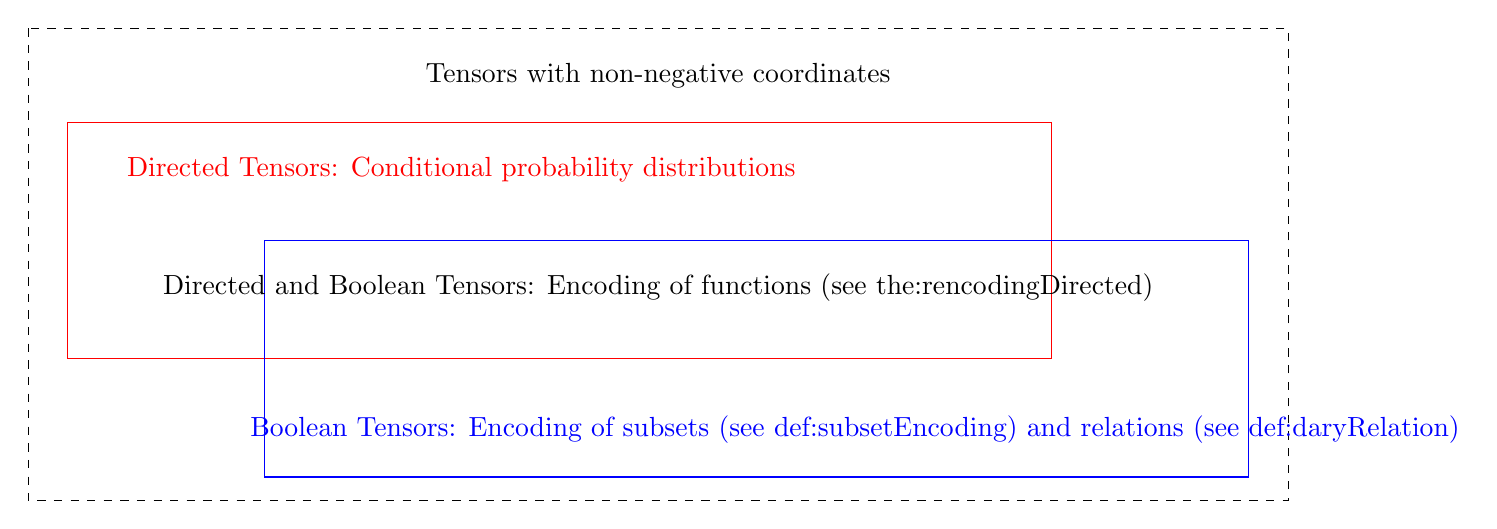
\begin{tikzpicture}[yscale=0.6]
	\draw[dashed] (-10.5,12) rectangle (5.5,2);
	\node[anchor=center] (text) at (-2.5,11) {Tensors with non-negative coordinates};
	
	\draw[red] (-10,10) rectangle (2.5,5); 
	\node[anchor=center,red] (text) at (-5,9) {Directed Tensors: Conditional probability distributions};
	\draw[blue] (-7.5,7.5) rectangle (5,2.5); 
	\node[anchor=center,blue] (text) at (0,3.5) {Boolean Tensors: Encoding of subsets (see \defref{def:subsetEncoding}) and relations (see \defref{def:daryRelation})};

	\node[anchor=center] (text) at (-2.5,6.5) {Directed and Boolean Tensors: Encoding of functions (see \theref{the:rencodingDirected})};
\end{tikzpicture}
    \end{center}
    \caption{Sketch of the tensors with non-negative coordinates.
    We investigate in this chapter tensors, which are directed and boolean.}\label{fig:dbTensorSketch}
\end{figure}

\sect{Efficient representation and reasoning}

\textbf{Efficient storage schemes} can be derived for tensors with specific properties, whereas generic tensor storage schemes suffer from the curse of dimensions.
In \charef{cha:sparseRepresentation} we investigate the efficient representation of tensors based on $\cpformat$ decompositions.
When restricting the allowed leg tensors in different ways, we show that relational databases can be utilized as sparse storage of tensors.

\textbf{Efficient executions of contractions} will be derived based on message-passing schemes in \charef{cha:messagePassing}.
They are in most generality derived from expectation propagation schemes in variational inference.

\textbf{Approximation schemes} to tensors are investigated in \charef{cha:approximation}.
Approximating formats are oriented on the efficient representation of the approximating tensor.